\begin{figure*}
	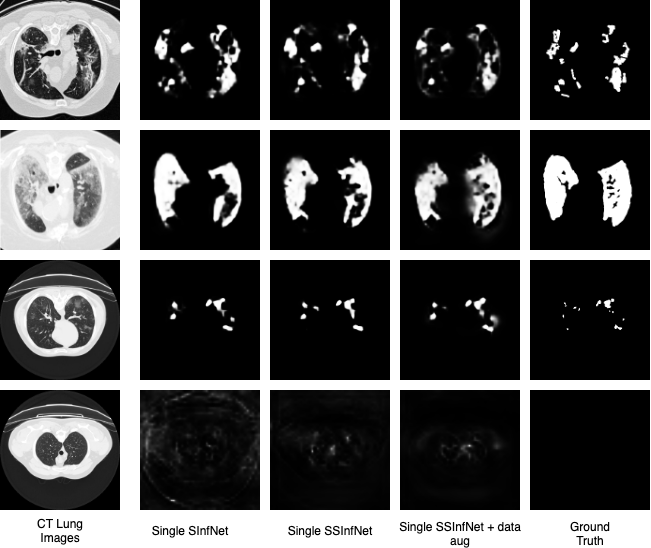
\includegraphics[width=\linewidth]{comparison_single.png}
	\caption{Comparison of single segmentation between different networks.}
	\label{fig:single-comparison}
\end{figure*}
\begin{figure*}
	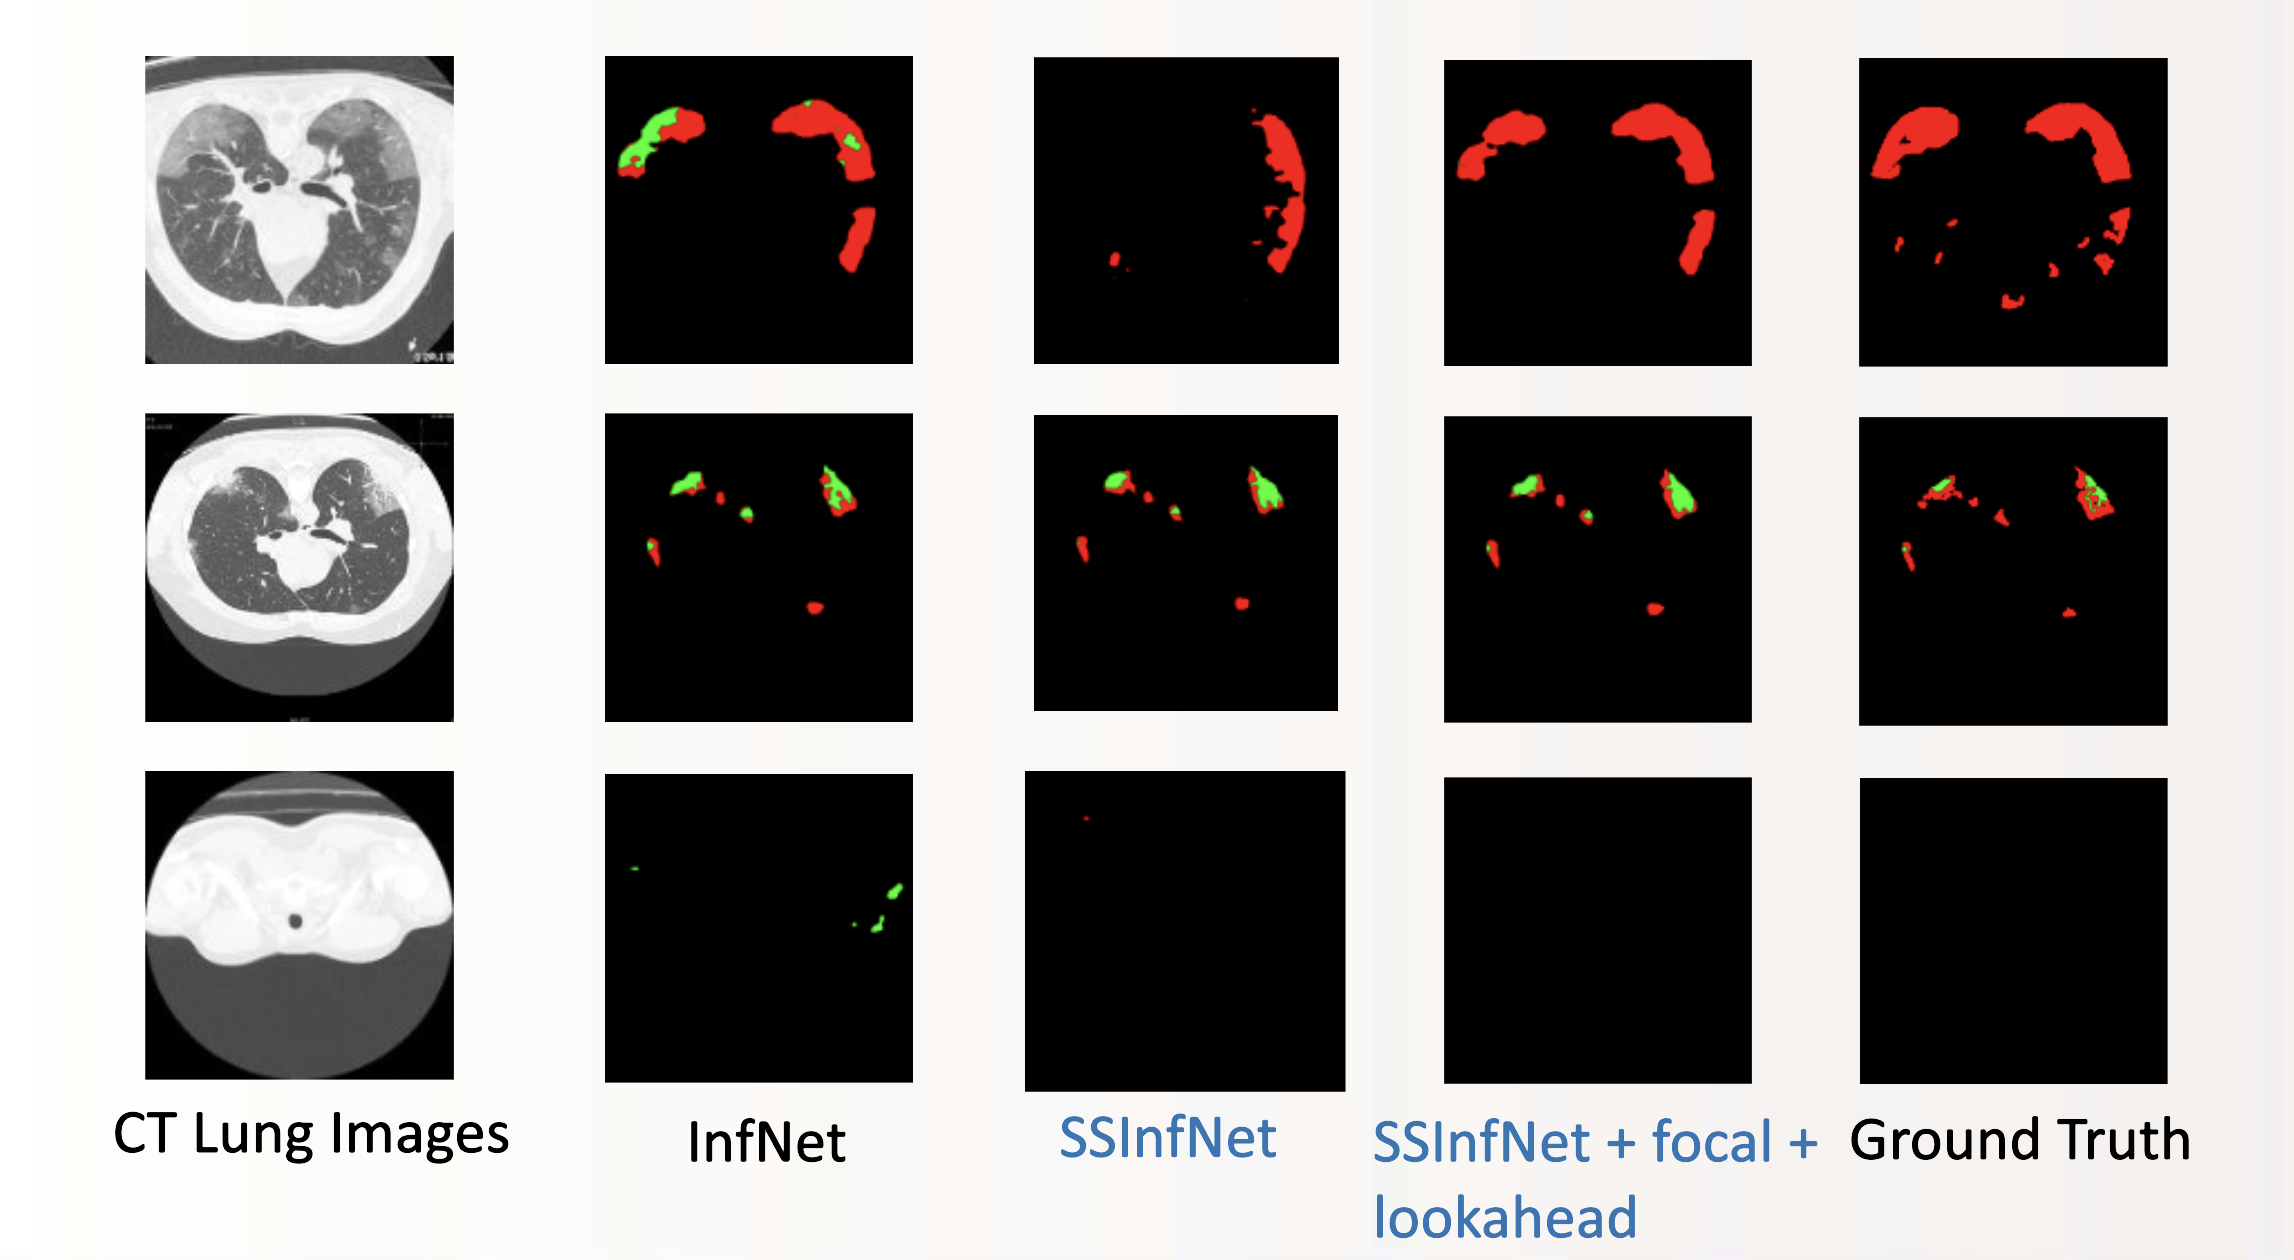
\includegraphics[width=\linewidth]{comparison_multi_weakprior.png}
	\caption{Comparison of multi segmentation between different networks with prior generated from single InfNet.}
	\label{fig:multi-weakprior-comparison}
\end{figure*}
\begin{figure*}
	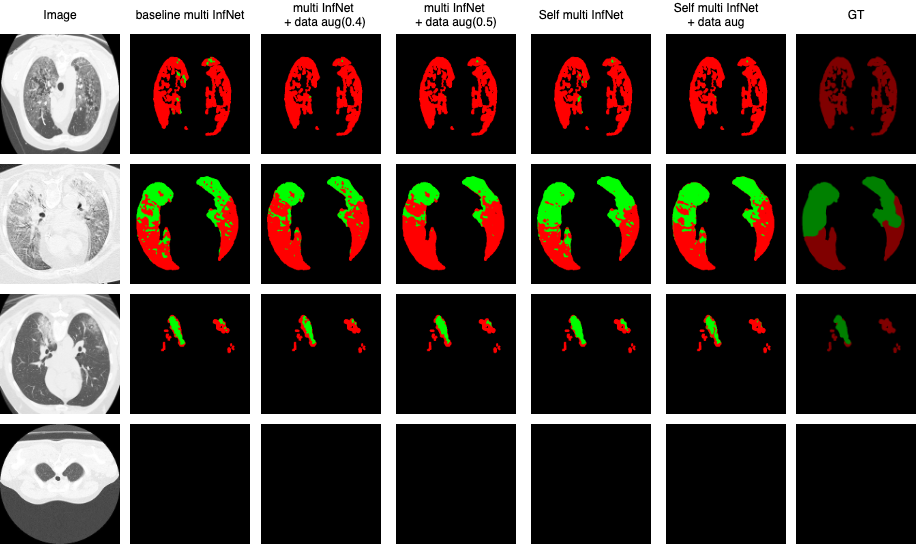
\includegraphics[width=\linewidth]{comparison_multi_strongprior.png}
	\caption{Comparison of multi segmentation between different networks with prior from Test Set.}
	\label{fig:multi-strongprior-comparison}
\end{figure*}

\begin{table}
	\begin{tabular}{|c||c|c|c|}
	\hline
	Method & F1 Score & Precision & Recall \\ \hline
	SInfNet & 0.28 & 0.28 & 0.28 \\ \hline
	SInfNet+data aug(0.4) & 0.61 & 0.61 & 0.61 \\ \hline
	SInfNet+data aug(0.5) & 0.42 & 0.42 & 0.42 \\ \hline
	Self SInfNet & 0.55 & 0.55 & 0.55 \\ \hline
	Self SInfNet+data aug & \textbf{0.62} & \textbf{0.62} & \textbf{0.62} \\ \hline
	\end{tabular}
	\caption{Table shows the result of severity score prediction on CT lung images using segmentation.}
	\label{tab:severity}
\end{table}

\section{Results}
In this section, we will show the results of our experiments obtained. We will divide this section into two different subsections: Result for self-supervised InfNet and result for estimation of severity score.

\subsection{Result for self-supervised InfNet}
 The result for our comparison between the baseline InfNet model and our self-supervised model can be seen in \ref{tab:single}, \ref{tab:multi-weakprior}, and \ref{tab:multi-strongprior}. The table is plotted with  several metrics: dice, jaccard, sensitvity, specificity, and mean absolute error (MAE). 
 
 For the table that contains mean and error, the mean are calculated as:
 \begin{equation}
mean =  \frac{\sum_{i=1}^{N}Metric(\hat{y_i}, y_i)}{N}
 \end{equation}
 Where Metric refers to either \textit{Dice, Jaccard, Sensitivity, Specificity, or mean absolute error (MAE).} N refers to the number of test data samples.
 The error is:
 \begin{equation}
error =  SE x 1.96
 \end{equation}
 where SE is the standard error of the test data samples for the metric multiplied by 1.96.
Note that Mean $\pm$Error is the 95\% confidence interval.
 
 We show several tables for our comparisons. \ref{tab:single} shows the result for the single segmentation InfNet. The single segmentation InfNet does not segment between ground-glass opacities or consolidation. The single segmentation will segment and represent all infected region as one. We can see that self-supervise can improve on the generalisation and consistency on predicting on the different CT lung images as they perform the best in terms of the error range. Even though the baseline single SInfNet performance have better mean values for dice, jaccard, and sensitivity, the self-supervised approach helps to create robustness and consistency in the model itself to better handle outliers. We can see the results of the single segmentation in \ref{fig:single-comparison}. We can see that the baseline single SInfNet overestimated the infected region of an outlier in the segmentation result in the figure in the last row. The baseline single SInfNet even with added data augmentation predicted some infected region in the CT lung images when the ground truth does not contain any infected region. The self-supervised SInfNet did a better job at predicting outlier's where its prediction is more closely related to the ground truth than the baseline single SInfNet.
 
 \ref{tab:multi-weakprior} shows the result for the comparison between multiple segmentation InfNet. As the multiple segmentation InfNet requires a CT lung image concatenate with a prior as input where the prior is the segmentation of the infected region of the CT lung without considering the location of ground-glass opacities or consolidation. The prior represents the infected region as a whole. For the result of this table, the prior is obtained from the single segmentation InfNet. Then the prior is fed into the multiple segmentation InfNet to obtain the result. We can see from the table that the self-supervised multi SInfNet does a better job at predicting multiple segmentation than the the baseline multi SInfNet even with when the baseline multi SInfNet has been added with data augmentation. Self-supervised helps to prevent loss of performance when the  prediction is needed to be transferred from one network to another network. In our case, the prediction is transferred from the single self-SInfNet as prior to the multi self-SInfNet.  Self-supervised also creates a more consistent and robust network to outliers. We can see the segmentation result in \ref{fig:multi-weakprior-comparison}. The self-supervised with data augmentation does not seem to improve the performance on the self-supervised multi InfNet. However, it does reduce the difference in the error variation between different CT lung images. This means that data augmentation helps to cover a wide variety of CT lung images to create a more consistent prediction. Similar to the single segmentation network, the self-supervised are able to predict output that is more closely related to the ground-truth when fed with CT lung images with different distribution as shown in the last row of the figure. The self-supervised multi SInfNet is also able to predict a better prediction on the consolidation on the CT lung images than the baseline models. Self-supervised learning also helps to improve the performance when the number of labels contain a small amount in the dataset. The labels on consolidation contains a smaller ratio when compared to the ground-glass opacities and non-infected region. Our self-supervised multi SInfNet was able to predict consolidation more accurately than the baseline multi SInfNet models.
   
 \ref{tab:multi-strongprior} Shows the result for the comparison between multiple segmentation InfNet. The prior fed into the multiple segmentation InfNet for this result is the ground truth prior obtained from the test set. For the result of this table, the prior is obtained from the test set. The prior is therefore the ground-truth of the segmentation of the single SInfNet. 
 We can see from the table that the muti self SInfNet is the best performing network compare to the rest of the network. We can see that data augmentation improves the consistency of the network. However, data augmentation does not neccessarily improve the performance of the network. Data augmentation makes a network more robust to outliers but does not necessarily improve the performance of the network in CT lung images. The self-supervised multi SInfNet improves the performance of the consolidation by a large amount especially in the jaccard metric. We can see the figure of the comparison between different multi segmentation SInfNet with strong prior (Priors that are obtained from the test dataset) in \ref{fig:multi-strongprior-comparison}.
 We can see that the self-supervised multi SInfNet does a better job at predicting consolidation - a label of a smaller amount than the rest of the labels in the dataset. Self-supervised learning helps to improve the performance of the network especially the labels that are of smaller amount compare to the rest of the labels. 


\subsection{Result for estimation of severity score}
\ref{tab:severity} shows the result of the severity score with different networks. We can see that having data augmentation improves the performance of the baseline InfNet in severity calculation. It achieves an F1 score of 0.61,  an amount of more than two times the performance of baseline InfNet network. Enabling a higher value of random cutout in the data augmentation seems to reduce the performance of the severity score calculation by a marginal amount. The result of baseline InfNet with data augmentation where the random cutout is set to 0.5 have an F1 score of 0.42 with severity calculation. As having a higher random cutout value improves the network capacity to predict the image inpainting of the CT lung images, the capacity for the network to generalize to other information is lost. Adding self-supervised learning to the baseline InfNet model improves the network performance to 0.55, the performance is still lower than the baseline InfNet with data augmentation but it is two times the performance of baseline InfNet. Our self-supervised InfNet with added data augmentation yields the best performing result. The self-supervised InfNet with added data augmentation achieves a result of 0.62. The combination of self-supervised learning and data augmentation helps the InfNet model to generalise to different tasks as both technique aids the model in learning detailed information about CT lung images and a more diverse CT lug images distribution.